\documentclass[12pt,oneside]{book}
\usepackage{amsmath}
\usepackage{amssymb}
\usepackage{makeidx}
\usepackage{graphicx}
\usepackage{latexsym}
\usepackage{hyperref}
\hypersetup{
	linktoc=all, 
	colorlinks,
	citecolor=black,
	filecolor=black,
	linkcolor=black,
	urlcolor=black
}
\usepackage{fancyhdr}
\pagestyle{fancy}
% with this we ensure that the chapter and section
% headings are in lowercase.
\renewcommand{\chaptermark}[1]{%
\markboth{#1}{}}
\renewcommand{\sectionmark}[1]{%
\markright{\thesection\ #1}}
\fancyhf{} % delete current header and footer
\fancyhead[LE,RO]{\bfseries\thepage}
\fancyhead[LO]{\bfseries\rightmark}
\fancyhead[RE]{\bfseries\leftmark}
\renewcommand{\headrulewidth}{0.5pt}
\renewcommand{\footrulewidth}{0pt}
\addtolength{\headheight}{0.5pt} % space for the rule
\fancypagestyle{plain}{%
\fancyhead{} % get rid of headers on plain pages
\renewcommand{\headrulewidth}{0pt} % and the line
}
\usepackage{xepersian}
\settextfont[Scale=1.1]{Nazli}%{XB Niloofar}
\setlatintextfont[Scale=1]{Ubuntu}
%\setdigitfont[Scale=1]{XB Zar}
\defpersianfont\Sayeh[Scale=1]{XB Kayhan Sayeh}


\title{
{\small به نام خدا\\}
\vspace{5cm}
اوبونتو برای تازه‌واردها\\}
\author{ساسان نمیریان\\
نوا اژدری\\
احمد صوفی محمودی\\\\\\
\lr{http://www.ubuntu-book.org}\\
\lr{info@ubuntu-book.org}
}

\begin{document}
\frontmatter
\maketitle

\newpage
\tableofcontents

\newpage
\chapter{مقدمه}
\emph{\lr{Ubuntu}} تنها یک سیستم عامل آزاد و متن‌باز  با بیش از ۲۰ میلیون کاربر در سرتاسر جهان نیست؛ اوبونتو یک فرهنگ است، یک خلاقیت بزرگ، یک پروژهٔ گروهی، در نوبهٔ خود مهم‌ترین و برجسته‌ترین. اوبونتو یک جامعه از مردم است.\\
اگر در حال خواندن این راهنما هستید، ممکن است تصمیم گرفته باشید که از فضای سیستم عامل‌هایی مانند \lr{Windows} و \lr{Mac OS X} دور شوید و یا شاید اخیراً اوبونتو را بر روی رایانهٔ‌تان نصب کرده‌اید، اما مطمئن نیستید که از کجا باید شروع کنید.\\
استفاده از یک سیستم عامل جدید می‌تواند ترسناک باشد، مخصوصاً وقتی که با کلمه‌های ناآشنا روبه‌رو می‌شوید. بسیاری از مردم با اصطلاحات فنی یک سیستم عامل آشنا نیستند و معتقدند که این مفاهیم برایشان خیلی پیشرفته است. در واقع این موضوع درست نیست. اوبونتو به راحتی نصب می‌شود و استفاده از آن ساده است. و از همه مهم‌تر این‌که: \emph{کاملاً آزاد و  رایگان است}.\\

این راهنما برای کسانی است که به تازگی استفاده از گنو/لینوکس را شروع کرده‌اند و این امکان را به آن‌ها می‌دهد که تمام ابزارهای موردنیاز را بشناسند و از آن‌ها به درستی استفاده کنند.\\
شما با خواندن این کتاب می‌آموزید که چگونه کارهای زیر را انجام دهید:
\begin{itemize}
\item نصب و راه‌اندازی اوبونتو بر روی رایانه‌ٔتان
\item پشتیبانی فنی در این محیط
\item درک فلسفهٔ اوبونتو
\item ایجاد وحدت در رابط میز کاربری
\item استفاده از نرم افزارهای سازگار با اوبونتو
\end{itemize}


\mainmatter
\chapter{معرفی اوبونتو}
قبل از اینکه شروع به نصب کنیم، بهتر است در مورد فلسفه و مفهوم کلی سیستم عامل اوبونتو صحبت کنیم.
\section{تعاریف کلی}
بهتر است قبل از پرداختن به اوبونتو، در مورد برخی تعاریف، مثل سیستم عامل و هسته، توضیح داده شود.
\subsection{سیستم عامل چیست؟}
سیستم عامل برنامه‌ای است که با سخت افزار ارتباط مستقیم دارد و امکان اجرای برنامه‌های کاربردی (Application) را روی بستر سخت‌افزاری ممکن می‌سازد.
\subsection{هسته چیست؟}
هسته نقش قسمت مرکزی و سطح پایین یک سیستم عامل را ایفا می‌کند و وظایفی مانند ارتباط با سخت‌افزار و بارگذاری درایورها را به دوش می‌کشد.
\subsubsection{لینوکس چیست؟}
برخلاف تصور خیلی از افراد، لینوکس تنها یک هسته با همان وظایف گفته شده است. بسیار کم پیش می‌آید که در کاربرد روزانه، به طور مستقیم با خود هستهٔ لینوکس ارتباط برقرار کنیم. با این حال، هسته نقش اصلی را در سیستم عامل بر عهده دارد.
\subsubsection{چرا گنو/لینوکس آری، لینوکس نه؟}
همان طور که گفته شد، لینوکس تنها یک هسته است و یک هسته به خودی خود، هیچ کاری نمی‌تواند برای ما انجام دهد. ما برای برطرف‌کردن نیازهای روزانه، به نرم‌افزارهای متعددی نیازمندیم. نرم‌افزارهایی که اکثراً از پروژهٔ گنو یا گرفته شده یا بر اساس فلسفهٔ نرم‌افزارهای آزاد و مجوز GNU GPL ساخته شده اند. برای همین، بهتر است این سیستم عامل (و نه خود هسته) را گنو/لینوکس بنامیم.
\subsubsection{توزیع گنو/لینوکس چیست؟}
گفتیم که پروژه گنو/لینوکس از پیوستن ابزارهای گنو و هستهٔ لینوکس به وجود آمد. حالا فرض کنید شما بخواهید آن را نصب کنید. چکار باید بکنید؟ در حالت قدیم، باید یک متخصص کامل یونیکس باشید: هسته را بگیرید و کمپایل کنید، بعد یک دیسک را فرمت کنید و بوت سکتور را طوری تنظیم کنید که از این کرنل بوت شود. سپس دستورات (برنامه‌های) دیگر را روی آن کپی کنید و تمام وابستگی‌ها را هم رعایت کنید. چنین کاری برای بیش‌تر کاربران بسیار سخت است.\\
برای حل این مشکل، افراد و شرکت‌هایی آمده‌اند و توزیع‌هایی (Distribution) را ساخته‌اند. در همان سال ۱۹۹۲ که هسته لینوکس آمد، توزیع‌ها هم ظاهر شدند. کاربران هسته را به همراه چند برنامه اصلی و یک برنامه نصب کننده روی یکی دو فلاپی جا می‌دادند و بین دیگران پخش می‌کردند.
\section{اوبونتو چیست؟}
اوبونتو (تلفظ به صورت \lr{|oo'boontoo|}) یک سیستم عامل کامل گنو/لینوکسی برای دسکتاپ است. اوبونتو همانند سایر گنو/لینوکس‌ها، آزاد است و دارای پشتیبانی از طرف جامعهٔ کاربری و پشتیبانی حرفه‌ای از طرف شرکت سازندهٔ آن، \lr{Canonical}، است.\\
\subsection{چطور اوبونتو  و لینوکس به هم مربوط‌اند؟}
اوبونتو یک سیستم عامل است که از لینوکس به عنوان هسته استفاده می‌کند. به طور ساده، لینوکس یک بخش از اوبونتو  است که وظیفهٔ مرکزی را به عهده دارد.\\

جامعهٔ اوبونتو، بر پایهٔ اندیشه‌های مطرح‌شده در بیانیهٔ اوبونتو فراهم آمده است. این‌که:

\begin{itemize}
\item نرم‌افزار باید رایگان باشد.
\item نرم‌افزارها باید در زبان محلی کاربران قابل استفاده باشند و معلولیت‌ها را پوشش دهد تا اوبونتو برای بیش‌ترین افراد ممکن مورد استفاده قرار گیرد.
\item کاربران باید آزادی تغییر نرم‌افزار به شیوهٔ دلخواه‌شان را داشته باشند.\\
\end{itemize}

برای همین، اوبونتو تنها یک سیستم عامل نیست و دارای سه بخش متفاوت است:

\begin{itemize}
\item فلسفه
\item پروژهٔ نرم‌افزار مشترک جهانی
\item سیستم عامل
\end{itemize}

این راهنما در تمام این مفاهیم در بخش های بعد گسترده می‌شود؛ اما در حال حاضر مهم‌ترین چیز که باید به خاطر داشته باشید این است که اوبونتو بیش‌تر از یک نرم افزار است.

\section{فلسفهٔ اوبونتو}
اوبونتو یک لغت قدیمی در زبان آفریقایی به معنای یک نفر برای همه یا انسانیت با دیگران است.\\
مجموعهٔ اوبونتو با سیستم عامل‌های دیگر متفاوت است؛ به دلیل اینکه روح انسانیت و جامعه را به دنیای رایانه می آورد. کاربران اوبونتو در یک باور عمیق هم‌عقیده‌اند که نرم‌افزار باید قابل دسترس برای همه انسان‌ها، با هر زبان و رنگ پوست، توانایی جسمی و درآمدی باشد.

\section{نرم‌افزار اختصاصی در مقابل نرم‌افزار آزاد و منبع‌باز}
نرم‌افزارهای اختصاصی، توسط یک شرکت طراحی می‌شوند، توسعه می‌یابند و فروخته می‌شوند. این نرم‌افزارها برای به‌دست‌آوردن سود فروخته می‌شوند و فقط بر روی یک نوع از کامپیوترها کاربرد دارند. برای مثال، سیستم عامل‌های اختصاصی مانند \lr{Microsoft Windows} و یا \lr{Mac OS X} را در نظر بگیرید. کد منبع این سیستم‌ها در دسترس نیست و اگر شما سعی به تغییر یا توزیع آن را داشته باشید، متهم خواهید شد.\\
اوبونتو، به عبارت دیگر یک نرم افزار اختصاصی نیست؛ به این دلیل که به صورت فعال توسط جامعه FOSS نگهداری می شود.

\subsection*{\lr{FOSS} چیست؟}
\lr{FOSS} مخفف عبارت \lr{Free/Libre Open Source Software} و به معنی نرم‌افزار آزاد و متن‌باز است. نرم افزار \lr{FOSS} به دلایل زیر با نرم افزارهای اختصاصی تفاوت دارد:

\begin{itemize}
\item استفادهٔ آزاد و رایگان
\item اشتراک‌گذاری آزاد و رایگان
\item توسعهٔ آزاد و رایگان
\end{itemize}

این یعنی شما بدون پرداخت هیچ مبلغی، می‌توانید اوبونتو را دانلود و استفاده کنید. شما می‌توانید به صورت کاملاً قانونی از سی‌دی/دی‌وی‌دی های اوبونتو به هر تعداد که می‌خواهید، کپی کرده و بین دوستان و آشنایان‌تان توزیع کنید. حتا کد منبع سیستم عامل اوبونتو آزادانه در دسترس شماست و می‌توانید آن را با توجه به نیازهای خود تغییر دهید.\\
اوبونتو از مجوز عمومی همگانی \lr{GNU}  (یا به طور ساده \lr{GPL}) استفاده می‌کند که به طور گسترده، در جامعهٔ \lr{FOSS} استفاده می شود. به همین دلیل، اوبونتو دارای آزادی‌هایی است که ذکر شد.\\
\lr{GPL} توسط بنیان‌گذار پروژهٔ گنو و بنیاد نرم‌افزارهای آزاد، ریچارد استالمن، در سال ۱۹۸۹ نوشته شد و به صراحت آمده است که کاربران برای اجرا، کپی، توزیع ، بازرسی، تغییر ، توسعه و بهبود نرم‌افزار ارائه‌شده آزاد هستند. گاهی \lr{GPL} با  نام مستعار کپی‌لفت (\lr{Copyleft}) می‌آید.

\subsection{چطور ممکن است اوبونتو رایگان باشد؟}
شما ممکن است تعجب کنید که در حال حاضر واقعاً چطور ممکن است اوبونتو رایگان باشد. آیا نکته و یا برخی هزینه‌های مخفی وجود دارد؟ به دو دلیل، اوبونتو رایگان است.\\
\begin{enumerate}
\item \textbf{مدیریت و بودجه‌بندی به پشتوانهٔ کنونیکال}\\
اگر چه  اوبونتو توسط جامعهٔ \lr{FOSS} نگهداری می‌شود، ولی مدیریت و بودجه از طریق شرکت خصوصی کنونیکال انجام می‌شود.\\
کنونیکال پشتیبانی‌های تجاری را برای شرکت‌ها تامین می‌کند و از این راه درآمد دارد. درآمد حاصل از این پشتیبانی، برای توسعهٔ مستمر اوبونتو مصرف می‌شود. این توسعهٔ مستمر، شامل موارد زیر است:
\begin{itemize}
\item انتشار نسخه های جدید اوبونتو هر شش ماه
\item به‌روزآوری‌های امنیتی
\item سرورهای میزبانی وب برای جامعهٔ آنلاین اوبونتو 
\item دفاتر کنونیکال
\end{itemize}
\item \textbf{اوبونتو از طریق جامعهٔ \lr{FOSS} نگهداری می‌شود}\\
از آنجایی که اوبونتو نرم‌افزاری کدباز است، کاربران برای دسترسی و تغییر کد منبع، آزاد هستند و این به بهتر شدن سیستم عامل برای همه کمک می‌کند.\\
اوبونتو هم یک جامعهٔ جهانی است و هم یک پروژهٔ نرم‌افزاری مشترک. مردم در سرتاسر جهان می‌توانند زمان و توانایی‌های خود را با هم به اشتراک بگذارند و در فعالیت‌هایی مانند زیر کمک کنند:
\begin{itemize}
\item تست اشکالات نرم‌افزار
\item ارسال مستندات کاربری
\item طراحی اثر هنری
\item ارائهٔ بازخورد
\item نگارش جملاتی زیبا دربارهٔ اوبونتو
\end{itemize}
\end{enumerate}

\section{چرا باید از اوبونتو استفاده کرد؟}
\begin{itemize}
\item[-] کار با اوبونتو ساده است.
\item[-] نصب نرم‌افزار، به‌روزرسانی سیستم عامل و پیدا کردن ابزارهای جدید با چند کلیک انجام پذیر است.
\item[-] محیط اصلی اوبونتو که یونیتی نام دارد، بسیار زیباست.
\item[-] آزاد است و برای همیشه رایگان باقی می‌ماند.
\item[-] اوبونتو با مشارکت کاربران‌اش ساخته شده و هرکسی می‌تواند برای بهتر شدن‌اش قدمی بردارد.
\item[-] اوبونتو از هستهٔ لینوکس استفاده می‌کند که طراحی بسیار منطقی و امنی دارد.
\item[-] اوبونتو به طور معمول، ویروس نمی‌گیرد.
\item[-] اوبونتو با اکثر رایانه‌ها و لپتاپ‌ها کار می‌کند و در بیش‌تر مواقع حتی نیاز به نصب یک درایور هم ندارید.
\item[-] با برنامه و فایل‌های فعلی‌تان سازگار است. اکثر محتوای چندرسانه‌ای در اوبونتو قابل پخش است و بسیاری از برنامه‌ها، مثل فایرفاکس، کروم و اسکایپ، نسخه‌ای مناسب اوبونتو دارند.
\item[-] پشتیبانی مناسب از بسیاری از زبان‌ها، از جمله زبان فارسی
\item[-] پایداری و سرعت بالا. اوبونتو کند نمی‌شود و لازم نیست هر چند وقت دوباره نصبش کنید. به چندین گیگابایت رَم هم برای اجرا نیاز ندارد.
\item[-] همیشه کسی برای کمک هست. اوبونتو در میان فارسی‌زبانان هم شناخته شده است و افراد زیادی در انجمن فارسی اوبونتو و کانال irc اوبونتوی فارسی، بدون هیچ چشم‌داشتی، به شما کمک می‌کنند.

\end{itemize}

\section{نکاتی در مورد اوبونتو}
کنونیکال نسخه‌های جدید اوبونتو را هر شش ماه یک بار، در ماه‌های آوریل و اکتبر، منتشر می‌کند. هر اوبونتو که منتشر می‌شود؛ یک شماره‌نسخه دارد که از سال و ماه انتشار آن تشکیل شده است. این راهنما به طور عمده برای اوبونتو ۱۳.۱۰ نوشته شده که در ماه اکتبر سال ۲۰۱۳ منتشر شده است.
علاوه بر شماره، هر نسخه اوبونتو یک نام هم دارد که از ترکیب یک صفت و نام یک حیوان تشکیل می‌شود. برای مثال نام کد برای اوبونتو ۱۳.۱۰، سمندر خوش‌مزه است.\\
یکی از بزرگترین ویژگی‌های اوبونتو این است که در داخل یک قاب زمان ساخته شده است. نسخه‌های جدید سیستم عامل هر شش ماه یک بار منتشر و معمولا پس از آن، به مدت ۱۸ ماه توسط کنونیکال پشتیبانی می‌شوند. این نسخه‌ها، به عنوان نسخه‌های عادی‌اند.
علاوه بر نسخه های عادی، کنونیکال پشتیبانی بلند مدت (\lr{LTS}) هم دارد که نسخه‌هایی از اوبونتو هستند که تقریبا هر دو سال یک بار (طبق زمان بندی) منتشر می‌شوند و برای ۵ سال بعد از آن پشتیبانی می‌شوند. آخرین نسخه با پشتیانی بلند مدت، اوبونتوی ۱۲.۰۴ است.

\chapter{نصب اوبونتو}
\section{دانلود و آماده‌سازی اولیه}
در این قسمت، با توجه به مشخصات سیستم خود، بین نسخه ۳۲ بیتی و ۶۴ بیتی نسخهٔ مناسب با معماری کامپیوترتان را از \href{http://www.ubuntu.com/download/desktop}{وب‌گاه اوبونتو} دانلود کنید. بعد از اتمام دانلود، ۲ روش برای نصب دارید: نصب از روی \lr{DVD} یا \lr{USB}.

\subsection[نحوهٔ رایت روی DVD]{نحوهٔ رایت روی \lr{DVD}}
بعد از دانلود \lr{ISO} ی مناسب، آن را روی یک دیسک نوری خام بنویسید. سیستم‌عامل‌های مختلف ابزارهای متفاوتی برای این کار دارند.

\subsubsection{در ویندوز}
در ویندوز می‌توان از \href{http://infrarecorder.org/}{\lr{InfraRecorder}} استفاده کرد.

\subsubsection{در \lr{Mac OS X}}
این سیستم عامل به صورت پیش‌فرض ابزار \lr{Disk Utility} را دارد که در مسیر:
\begin{center}
\lr{Disk Utility} \textsf{→} \lr{Utilities} \textsf{→} \lr{Applications}\\
\end{center}
قابل دسترس است. ابزار \lr{Disk Utility} را اجرا و \lr{ISO} را به قاب سمت چپ بکشید. بعد از زدن تیک \lr{Verify burned data}، روی \lr{Burn} کلیک کنید.

\subsubsection{در گنو/لینوکس}
کاربران گنو/لینوکس نیز می‌توانند از \lr{Brasero} یا \lr{K3b} استفاده کنند.

\subsection[نحوهٔ نصب بر روی USB]{نحوهٔ نصب بر روی \lr{USB}}
\subsubsection{در ویندوز}
می‌توان از \href{http://www.pendrivelinux.com/}{\lr{Pen Drive Linux}} یا \href{http://www.linuxliveusb.com/}{\lr{LiLi}} استفاده کرد. کار با این ابزارها بسیار ساده است. نوع توزیع (اوبونتو) و محل فایل \lr{ISO} دانلود شده را به نرم‌افزار بدهید و درایو حافظهٔ فلش را مشخص کنید.

\begin{center}
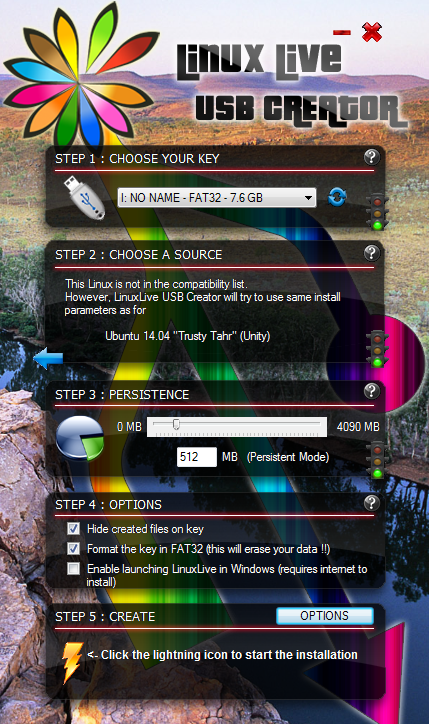
\includegraphics[scale=0.6]{pics/1.png}\\
\end{center}

\subsubsection{در \lr{Mac OS X}}
به کاربران \lr{OS X} توصیه می‌شود که از \lr{CD} یا \lr{DVD} استفاده کنند. زیرا رایانهٔ \lr{OS X} آن‌ها قابلیت راه‌اندازی از راه فایل‌های \lr{ISO} را ندارد.

\subsubsection{در گنو/لینوکس}
می‌توان از \lr{Unebootin} (روی تمام توزیع‌ها) و یا \lr{Ubuntu Startup Disk Creator} (مخصوص اوبونتو) استفاده کرد.

\begin{center}
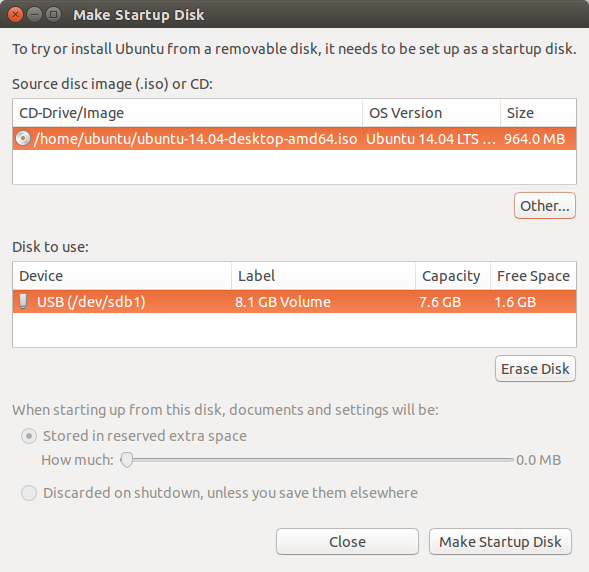
\includegraphics[scale=0.6]{pics/2.png}\\
\end{center}

\section{نصب و راه‌اندازی}
بعد از ریختن اوبونتو روی \lr{DVD} یا \lr{USB}، باید آن را بوت کنید. برای بوت‌کردن از راه دی‌وی‌دی یا یواس‌بی، باید به دفترچهٔ مادربورد رایانهٔ‌تان مراجعه کنید یا در اینترنت جست‌وجو کنید.\\
بعد از اینکه رایانه را با اوبونتو بوت کردید، دو انتخاب پیش‌رو دارید: انتخاب اول، نصب اوبونتو و انتخاب دوم، امتحان‌کردن اوبونتو است. با انتخاب گزینهٔ دوم، شما در هر زمان که تمایل به نصب داشتید می‌توانید با کلیک بر روی آیکون نصب اوبونتو آن را نصب کنید.
\begin{center}
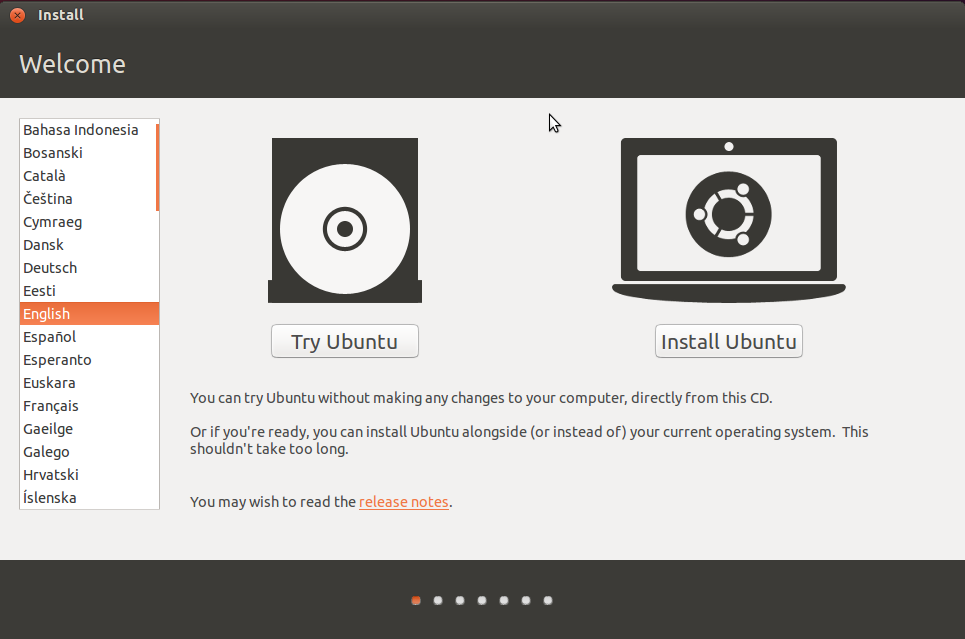
\includegraphics[scale=0.47]{pics/3.png}\\
\end{center}
در گام بعد، در صورتی که به اینترنت وصل نشده باشید و رایانهٔ‌تان دارای کارت شبکهٔ بی‌سیم باشد، شبکه‌های بی‌سیم موجود به شما نشان داده می‌شود که می‌توانید از همان‌جا شبکهٔ موردنظرتان را انتخاب کنید و به آن وصل شوید.
\begin{center}
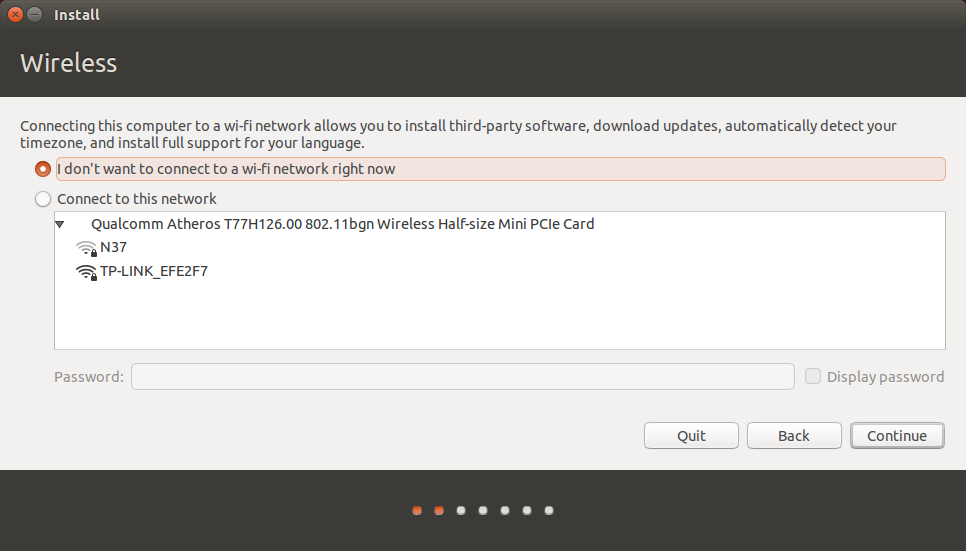
\includegraphics[scale=0.47]{pics/4.png}\\
\end{center}

در مرحلهٔ سوم، اطلاعاتی کلی مثل میزان فضای خالی سیستم‌تان و وصل‌بودن به اینترنت یا منبع برق را به شما نشان می‌دهد. همچنین در این مرحله می‌توانید با زدن تیک گزینهٔ \lr{Download updates while installing} آخرین به‌روزرسانی‌های اوبونتو را ضمن نصب دریافت و نصب کنید و با انتخاب \lr{Install this third-party software} کُدک‌های لازم برای پخش فایل‌های \lr{MP3} را نصب کنید.

\begin{center}
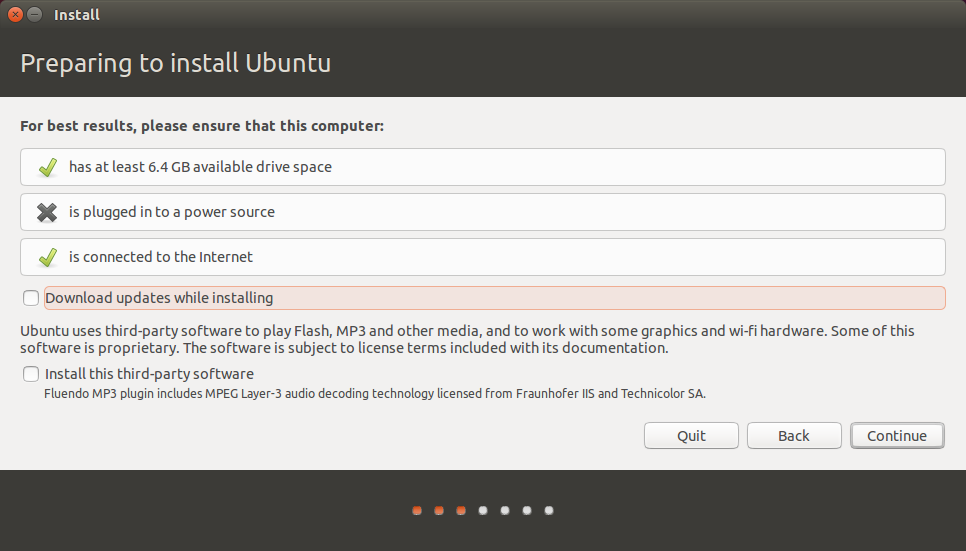
\includegraphics[scale=0.5]{pics/5.png}\\
\end{center}

در بخش بعد اوبونتو به شما چند انتخاب می‌دهد.
\begin{description}
\item[انتخاب اول]: نصب اوبونتو در کنار سیستم عامل فعلی\\
اگر دستگاه شما به اندازهٔ کافی (حداقل ۸ گیگابایت) فضای خالی داشته باشد، این گزینه برای شما نمایش داده می‌شود و اوبونتو به میزان دلخواه خودش، بخشی از فضای خالی روی هارد شما را به خودش اختصاص می دهد.

\item[انتخاب دوم]: پاک کردن سیستم عامل فعلی و نصب اوبونتو به جای آن\\
اگر دیگر تمایلی به استفاده از سیستم عامل فعلی خودتان ندارید، می‌توانید با انتخاب این گزینه اوبونتو را به جای آن جایگزین کنید. توجه داشته باشید که در صورت انتخاب این گزینه، تمام اطلاعات شما پاک خواهد شد.

\item[انتخاب سوم]: تنظیمات دستی (\lr{Something Else})\\
در این قسمت شما می‌توانید تنظیمات دلخواه خودتان را داشته باشید؛ مثلا یکی از پارتیشن‌های خود را پاک کرده و به اوبونتو اختصاص دهید.\\
\begin{center}
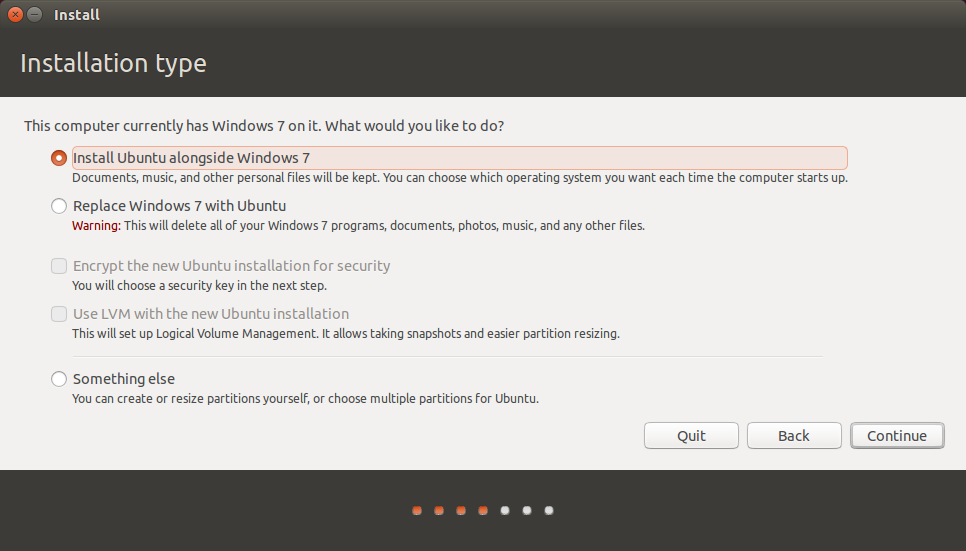
\includegraphics[scale=0.5]{pics/6.png}\\
\end{center}
* اگر فضای خالی ندارید و به پاک‌کردن یکی  از پارتیشن‌هایتان نیز متمایل نیستید، می‌توانید از فضای نصب خارج شده و در بخش امتحان زنده اوبونتو با برنامهٔ \lr{GParted} بخشی از فضای خالی پارتیشن  دلخواه خود را انتخاب کنید و آن را از پارتیشن جدا کنید و یا این‌که این کار را با برنامه‌های مخصوص کار با پارتیشن‌ها در سیستم عامل فعلی‌تان انجام دهید.
\end{description}

اوبونتو به حداقل ۲ پارتیشن احتیاج دارد: اولی پارتیشن اصلی و دیگری پارتیشنی برای حافظهٔ مجازی.\\
برای اضافه‌کردن حافظهٔ مجازی، شما باید روی \lr{+} (\lr{Add}) کلیک کنید و در بخش نوع پارتیشن (\lr{Type for the new partition}) گزینهٔ \lr{Logical} را انتخاب کنید. در بخش \lr{New partition size in megabytes} هم میزان فضایی تقریبا برابر با رم دستگاه یا کمی بیش‌تر را بدهید و در بخش \lr{Use as}، گزینهٔ \lr{swap area} را انتخاب کنید. \lr{OK} را بزنید.\\
برای اضافه‌کردن پارتیشن بعدی، روی فضای خالی باقی‌مانده کلیک کنید و \lr{+} (\lr{Add}) را بزنید. در بخش نوع پارتیشن \lr{Primary} و در بخش \lr{Use as}، ترجیحاً \lr{Ext4} را انتخاب کنید. در قسمت \lr{Mount point} هم گزینهٔ \lr{/} را برگزینید.\\
\begin{center}
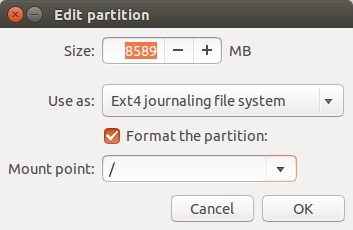
\includegraphics[scale=0.6]{pics/7.png}\\
\end{center}
پس از انجام این کارها، روی گزینهٔ \lr{Install Now} کلیک کنید تا اوبونتو شروع به نصب‌شدن کند.

\begin{center}
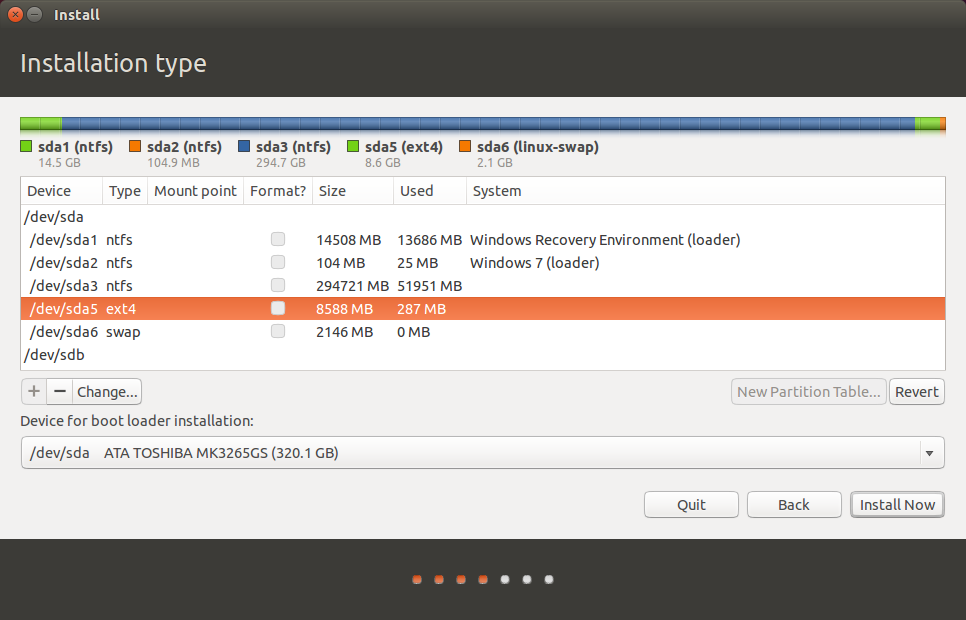
\includegraphics[scale=0.5]{pics/8.png}\\
\end{center}

در بخش بعد، روی محل زندگی خود در نقشه کلیک کنید تا زمان کامپیوتر را تنظیم کنید.\\
\begin{center}
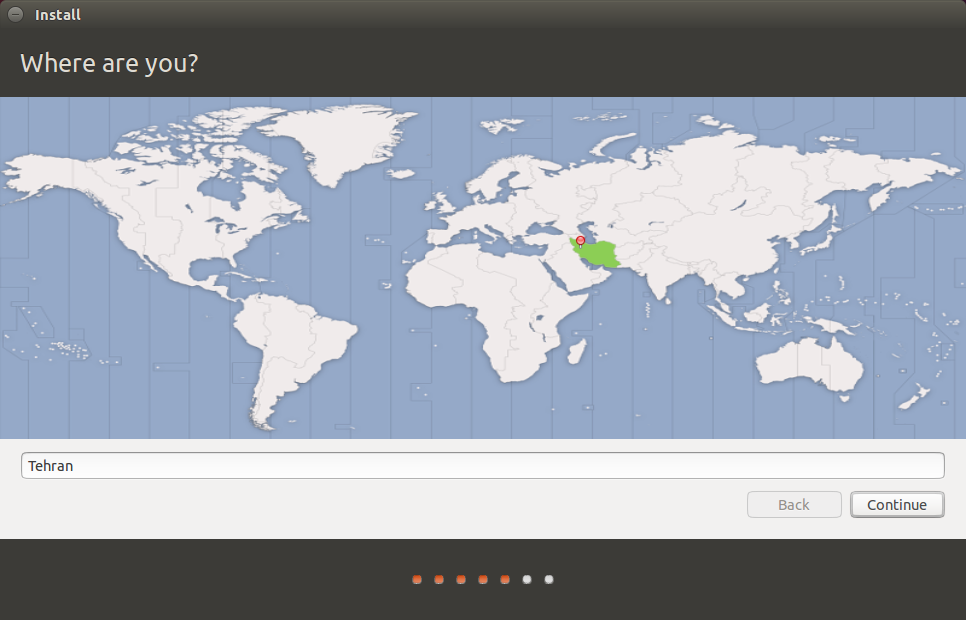
\includegraphics[scale=0.47]{pics/9.png}\\
\end{center}
در بخش بعد زبان \lr{Persian} را انتخاب کنید و روی ادامه (\lr{Continue}) کلیک کنید.

\begin{center}
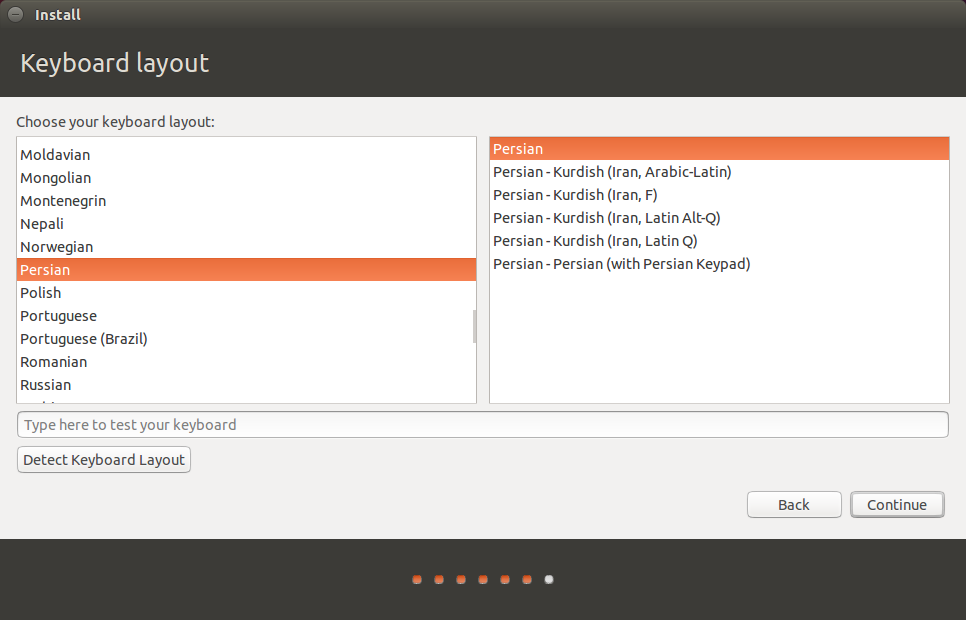
\includegraphics[scale=0.47]{pics/10.png}\\
\end{center}

در این قسمت مشخصات کاربری خود همراه با گذرواژه را وارد کنید.
\begin{center}
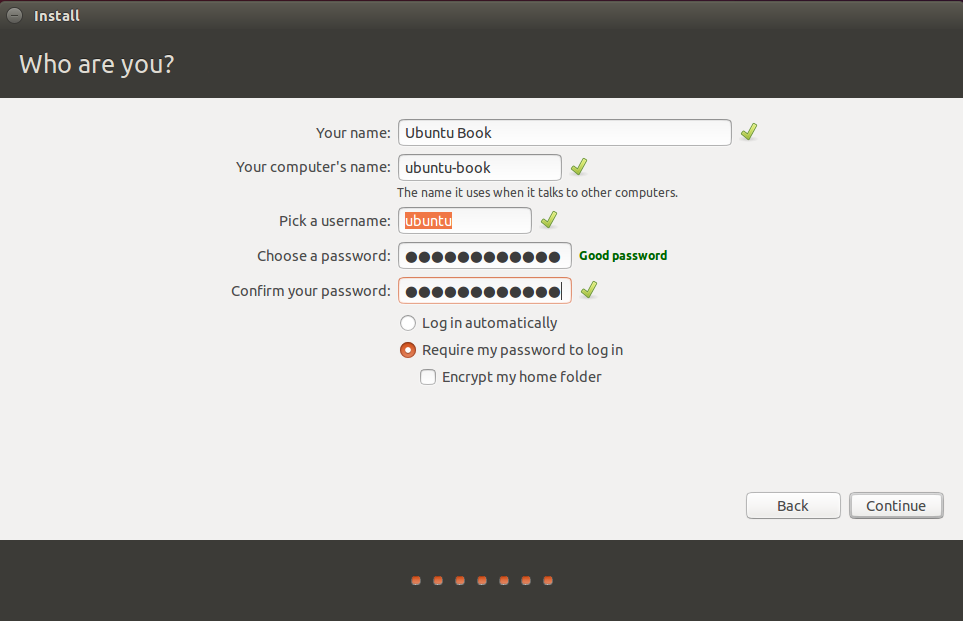
\includegraphics[scale=0.47]{pics/11.png}
\end{center}

اوبونتو خیلی سریع نصب خواهد شد. شما می‌توانید در این فرصت توضیحات مربوط به اوبونتو را مطالعه کنید تا نصب تمام شود.
\begin{center}
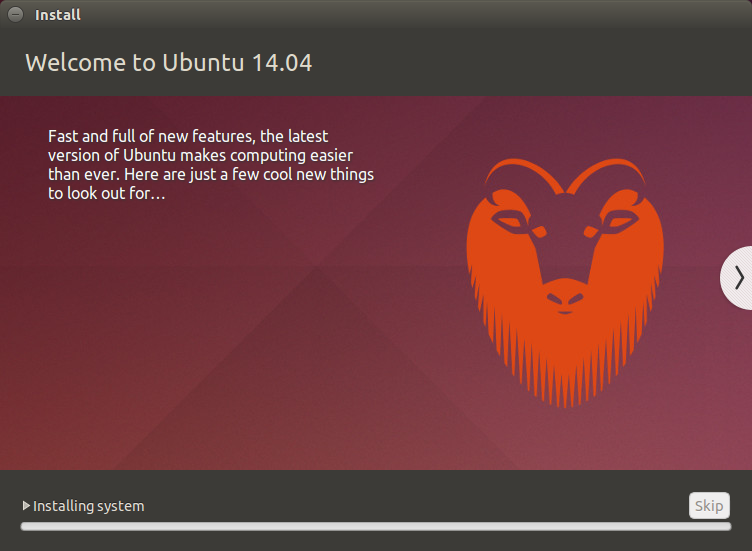
\includegraphics[scale=0.52]{pics/12.png}
\end{center}

\chapter{شروع کار با یونیتی}
حالا شما مراحل نصب را پشت سر گذاشته‌اید و اگر پا به پای این کتاب پیش رفته باشید، در صفحهٔ ورود اوبونتو قرار دارید.
\begin{center}
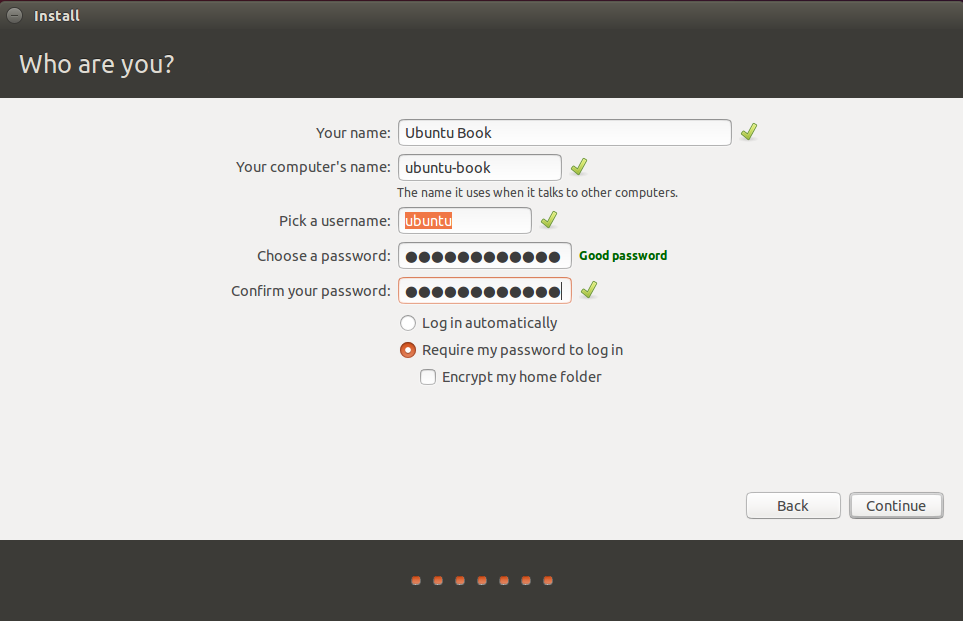
\includegraphics[scale=0.4]{pics/11.jpg}
\end{center}

بعد از واردکردن گذرواژه، وارد صفحهٔ زیر می‌شوید. این همان یونیتی است؛ محیطی که به طور پیش‌فرض در اوبونتو با آن کار خواهید کرد.
\begin{center}
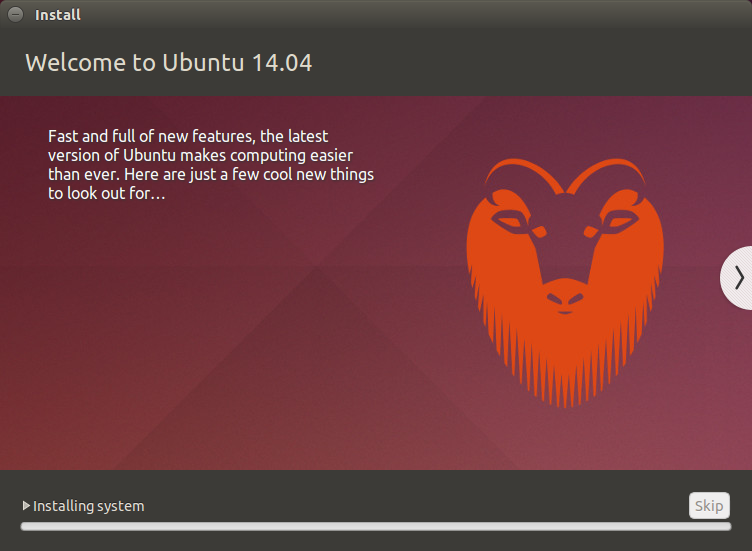
\includegraphics[scale=0.4]{pics/12.jpg}
\end{center}

\section{یونیتی چیست؟}
یونیتی محیطی است که سادگی، زیبایی، قدرت و یکپارچگی را هم برای کاربران و هم برای توسعه دهندگان نرم‌افزار فراهم می‌کند.
هیچ جای نگرانی نیست؛ یونیتی تماماً ویژگی‌های محیط‌های قبلی را که با آن‌ها احتمالاً در ویندوز یا سیستم عامل اپل کار کرده‌اید، دارد. ویژگی‌هایی مانند کشیدن و رهاکردن، کلیک‌کردن روی آیکون‌ها، قابلیت کپی‌کردن و بسیاری دیگر.
در ادامه بیش‌تر با یونیتی آشنا خواهید شد.
\subsection{تاریخچهٔ یونیتی}
شاید برای‌تان جالب باشد که یونیتی از کجا آمده است، چه گروهی آن را توسعه می‌دهند و از ابتدا روی اوبونتو بوده است.\\
یونیتی محیط کاری است که در حال حاضر تنها روی توزیع اوبونتو در دسترس است و توسط تیم اوبونتو در حال توسعه است. یونیتی یکی از جوان ترین محیط‌های کاری است. در‌واقع، یونیتی از توزیع ۱۱/۰۴ روی اوبونتو قرار گرفت و عمری کمتر از ۳ سال دارد؛ اما توانسته در همین مدت کوتاه، محیطی بسیار ساده، زیبا و کارآمد را به کاربران خود ارائه دهد. یونیتی با هدفِ رفتن اوبونتو بر روی دستگاه‌های دیگر (تبلت‌ها و گوشی‌ها و تلویزیون‌های هوشمند) و ظاهری یکپارچه برای تمامی دستگاه‌ها طراحی شده است و در هر نسخه، به ویژگی‌ها و پایداری آن افزوده می‌شود. اوبونتو ۱۳/۱۰ از نسخه ۷ یونیتی استفاده می‌کند.
\section{واسط کاربری یونیتی}
ظاهر یونیتی شامل بخش‌های زیر است:
\begin{itemize}
\item میزکار
\item اجراگر (\lr{Launcher})
\item پنل
\item داشبورد
\item هود
\end{itemize}

\subsection{میزکار}
محیط اصلی شماست. در این محیط، شما می‌توانید برنامه‌ها و پنجره‌های مختلف را باز یا بسته کنید.
\subsection[اجراگر (Launcher)]{اجراگر (\lr{Launcher})}
اجراگر همان سکویی است که در سمت چپ به صورت عمودی قابل مشاهده است. در لانچر، تمام برنامه‌های باز شما نمایش داده می‌شود. همچنین شما می‌توانید برنامه‌هایی را که بیش‌تر به آن‌ها نیاز دارید، در آن‌جا نگه دارید تا با سرعت بیش‌تری به آن‌ها دسترسی داشته باشید.
\subsubsection{راهنمای اجراگر}
برای اضافه و حذف کردن آیکن یک برنامه به اجراگر، کافی است روی لوگوی اوبونتو کلیک کنید و نام یا ویژگی برنامهٔ مورد نظر خود را تایپ کنید و بعد، آیکن آن برنامه را با موس گرفته و به روی اجراگر بکشید و رهایش کنید. برای حذف‌کردن نیز تنها کافیست روی آن آیکن، کلیک راست موس را بزنید و روی \lr{Unlock from Launcher} کلیک کنید؛ یا این‌که آیکن را گرفته و آن را بر روی آیکن سطل زباله برده و رها کنید تا آیکن برنامه از اجراگر حذف شود.
\subsection{هود}
فرایند گشتن در منوهای تودرتو و پیچیده و به خاطر سپردن موقعیت زیرمنوها، همیشه کاری بیهوده و زمانبر بوده است. یونیتی با هود به شما امکان جست‌و‌جوی سریع و بی‌دردسر را در منوها می‌دهد. با زدن کلید \lr{Alt} در پنجرهٔ برنامهٔ در حال اجرا، \lr{Hud} را فعال کرده و در منوهای آن پنجره جست‌وجو کنید.
\begin{center}
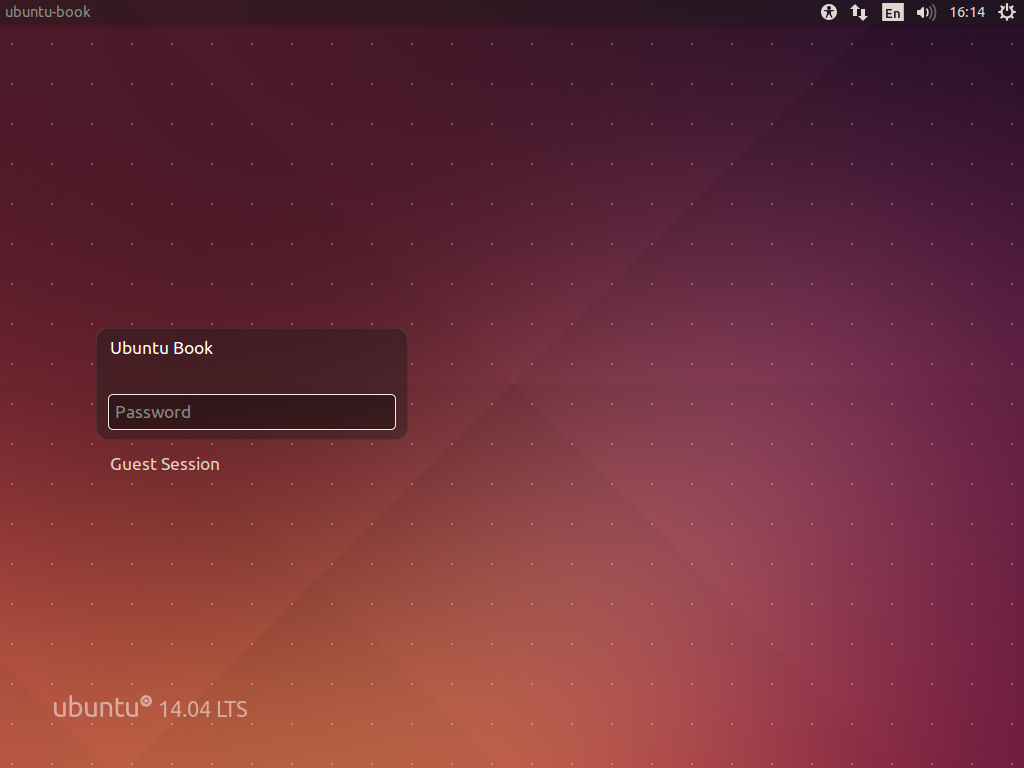
\includegraphics[scale=0.43]{pics/13.jpg}
\end{center}

\subsection{پنل}
پنل همان نواری است که در بالاترین قسمت از محیط خود آن را می‌بینید. در پنل، اطلاعاتی مانند منوی تنظیمات، ساعت و تاریخ ، صدا، شبکه و منوی من که برای اطلاع از آخرین وضیعت پیام‌های پست الکترونیکی و شبکه‌های اجتماعی و چت با دوستان‌تان است. اما شاید مهم‌ترین چیزی که در پنل به آن نیاز دارید، منوی پنجره‌ای است که در آن مشغول به کار هستید.

\subsubsection{ویژگی‌های پنل}
پنل از دو بخش تشکیل شده است: بخش سمت راست که در آن منوی تنظیمات، منوی کاربر، ساعت و تاریخ، تنظیمات صدا، تنظیمات شبکه، منوی من، نمایش باتری (در صورت استفاده از لپ‌تاپ) و تغییر زبان قرار گرفته و در سمت چپ، منوی برنامه وجود دارد که ابتدا نام پنجره فعال در آن نمایان است؛ اما با بردن موس بر روی سمت چپ پنل، این منو نمایان می‌شود. این قابلیت یونیتی باعث می‌شود که وقتی به منو احتیاجی ندارید، از دید پنهان باشد.
\begin{description}
\item[منوی من] \hfill \\
در منوی من که به شکل یک پاکت نامه در بالا نمایان است، به موارد زیر دسترسی خواهید داشت:
\begin{itemize}
\item نوع وضعیت در برنامه‌های گفت‌وگو (چت)
\item دسترسی و مدیریت حساب‌های شبکه‌های اجتماعی
\item دسترسی و مدیریت پست الکترونیکی
\item دسترسی به برنامه‌های تحت وب نصب‌شدهٔ مرتبط
\end{itemize}
این پاکت نامه، در صورتی که پیغامی خوانده نشده داشته باشید، به رنگ آبی در می آید. همچنین شما می توانید با کلیک وسط موس روی این پاکت نامه، به نشانه اطلاع‌تان از پیغام، رنگ‌اش را به رنگ اولیه تغییر دهید.
\begin{center}
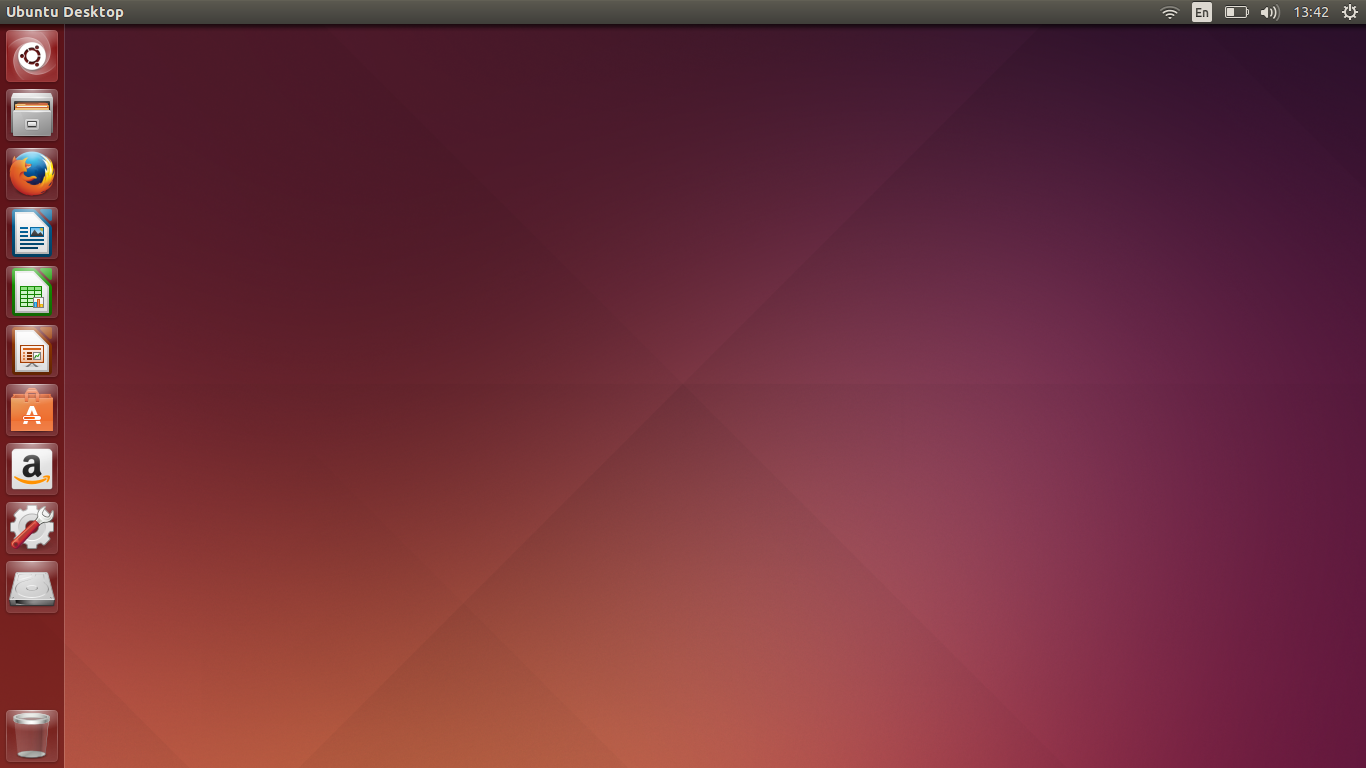
\includegraphics[scale=0.43]{pics/14.jpg}
\end{center}

\item[نشانگر شبکه] \hfill \\
شما در این منو می‌توانید شبکهٔ بی‌سیم خود را انتخاب کنید و با وارد کردن گذرواژه، از این شبکه بی‌سیم استفاده کنید. همچنین، این منو دسترسی سریع شما را به تنظیمات شبکه و \lr{VPN} فراهم می‌کند.
\begin{center}
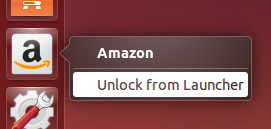
\includegraphics[scale=0.43]{pics/15.jpg}
\end{center}

\item[نشانگر صدا] \hfill \\
در این نشانگر، قادر خوهید بود صدا را کم یا زیاد کنید. همچنین امکان پخش و یا تغییر آهنگ در حال پخش نیز وجود دارد.
\begin{center}
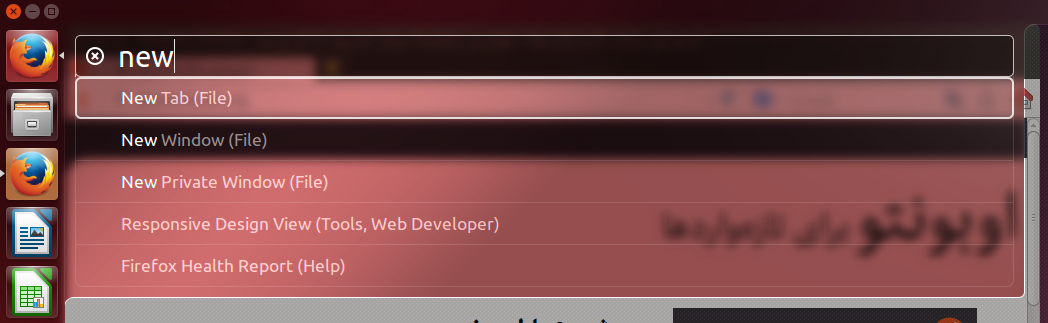
\includegraphics[scale=0.43]{pics/16.jpg}
\end{center}

\item[نشانگر ساعت] \hfill \\
در این نشانگر شما به تنظیمات ساعت، تاریخ و تقویم ماهانه دسترسی خواهید داشت.
\begin{center}

\includegraphics[scale=0.43]{pics/17.jpg}
\end{center}

\item[نشانگر تنظیمات] \hfill \\
شما در این نشانگر، به تنظیمات صفحه نمایش، تنظیمات سیستم، بروزرسانی، چاپگر و خاموش کردن یا شروع مجدد سیستم و سوییچ‌کردن از یک حساب کاربری به حساب کاربری دیگر دسترسی دارید.
\begin{center}
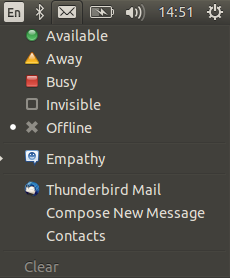
\includegraphics[scale=0.43]{pics/18.jpg}
\end{center}

\end{description}

\subsection{داشبورد}
داشبورد واسطی است که سریع‌ترین و راحت‌ترین دسترسی به فایل‌ها و برنامه‌ها را برای کاربران فراهم می‌کند. شما به کمک داشبورد می‌توانید نام برنامه یا کلمهٔ کلیدی آن را جست‌وجو کنید. همچنین می‌توانید برای جست‌وجوی خود، محدودیت‌هایی را اعمال کنید تا فقط در آن دسته به دنبال نتیجه باشید. همچنین با بازشدن داشبورد، به فایل‌ها و برنامه‌هایی که به تازگی استفاده کرده‌اید، دسترسی خواهید داشت.
\begin{center}
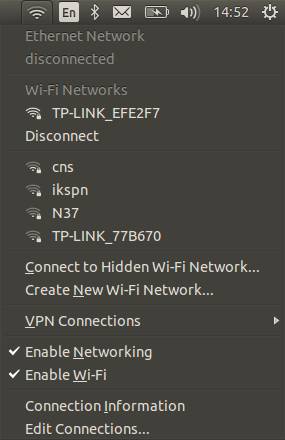
\includegraphics[scale=0.43]{pics/19.jpg}
\end{center}

\subsubsection{نحوهٔ دسترسی به داشبورد}
شما برای دسترسی به داشبورد، می‌توانید از ۲ راه استفاده کنید؛ راه اول این‌که می‌توانید با استفاده از موس، روی بالاترین آیکون در لانچر (آیکون اوبونتو) کلیک کنید و داشبورد نمایان خواهد شد. همچنین می‌توانید در کیبورد روی دکمهٔ ویژه (که دکمهٔ ویندوز هم نامیده می‌شود) کلیک کنید تا داشبورد نمایان شود.

\subsubsection{ظاهر داشبورد}
داشبورد از بخش‌های زیر تشکیل شده است:
\begin{itemize}
\item جست‌وجو
\item نمایشگر
\item فیلتر
\item \textbf{لنزها}\\
دش به طور پیش فرض ۶ لنز دارد که هر لنز، برای دسترسی سریع‌تر شما به هدف‌تان طراحی شده است. این ۶ لنز عبارت‌اند از: لنز خانه که امکان دسترسی به آخرین فایل‌ها و برنامه‌ها را دارد، لنز برنامه که تنها برای نرم‌افزارهاست، لنز فایل که تنها بین فایل‌های شما جست‌وجو می کند، لنز موسیقی که فایل‌ها موسیقی شما را پیدا می‌کند، لنز عکس بین عکس‌های شما می گردد و همین‌طور لنز فیلم که بین فیلم‌هایی که روی دستگاه شما قرار دارد و فیلم‌هایی که با آن موضوع در فضای اینترنت قرار دارد، جست‌وجو را انجام می‌دهد.
\end{itemize}

\subsubsection{پیش‌نمایش}
امکان مشاهدهٔ پیش‌نمایشی از محتواهای مختلف، با کلیک راست روی آن در داشبورد وجود دارد. مثلا با کلیک راست روی آیکن \lr{Chromium} در داشبورد، توضیحاتی از آن به همراه اسکرین‌شات و امتیاز کسب‌شده از کاربران نشان داده می‌شود. پیش‌نمایش از برنامه‌ها، تصاویر، ویدیو، موزیک و تعدادی دیگر از قالب ها پشتیبانی می‌کند.

\subsection{برنامه‌های تحت وب}
با کمک برنامه‌های تحت وب یا \lr{WebApps}، می‌توان وب‌سایت‌هایی مانند \lr{Gmail}، \lr{Grooveshark}، \lr{Last.fm}، \lr{Facebook} و بسیاری دیگر را با محیط \lr{Unity} یکپارچه کرد. برای مثال با نصب \lr{WebApp}های مناسب، می‌توانید \lr{Grooveshark} را با منو صدا کنترل و پیام ها جدید \lr{Google+}‎ را با سیستم اعلان اوبونتو دریافت نمایید. دو \lr{WebApp} فروشگاه موسیقی \lr{Ubuntu One} و \lr{Amazon}، به صورت پیش‌فرض فعال هستند. \lr{WebApp} های بیش‌تر، از مرکز نرم‌افزاری قابل نصب هستند؛ اما راه راحت‌تر آن است که با مرورگر \lr{Firefox}، سایت مورد نظر خود را، مانند \lr{Gmail}، باز کنید که بعد از آن، پیشنهاد نصب (در صورت موجود بودن برنامه برای آن وب‌سایت) به شما داده می‌شود.

\chapter{کارهای بعد از نصب}
\section{بررسی نکات انتشار}
 اوبونتو در هر نسخه پیشرفت‌های بسیاری می‌کند. آیا با پیشرفت‌های اوبونتوی ۱۳/۱۰ آشنا هستید؟ همین الان نکات انتشار اوبونتو را مطالعه کنید.

\section{نصب درایورها}
اگر از یک کاربر ویندوز بپرسید بعد از نصب ویندوز، نوبت چیست، بدون شک جواب خواهد داد: «نصب درایور»! اکثر کاربرانی که از ویندوز به سمت اوبونتو کشیده می‌شوند، در اوایل به فکر دانلود و نصب درایورها هستند!\\
در اوبونتو عمدتاً نیاز به نصب درایور خارجی ندارید و این سیستم عامل، بیش‌تر درایوهای مورد نیاز را به همراه دارد. اوبونتو را به صورت زنده بوت کنید و اگر همه چیز کار می‌کرد (صدا داشتید و صفحات وب را به خوبی توانستید مرور کنید)، آن را نصب کنید.\\
فقط ممکن است این احتمال وجود داشته باشد که اوبونتو بعضی از سخت‌افزارها، مثل کارت شبکه بی‌سیم را شناسایی نکند یا برای کارایی بیش‌تر گرافیکی، نیاز به نصب درایورهای انحصاری باشد.\\
برای نصب این درایورها، از \lr{System Settings}، گزینهٔ \lr{Software Sources} را انتخاب کنید و روی تب \lr{Additional Drivers} کلیک کنید. این ابزار سعی می‌کند برای سخت‌افزارهایی که شناخته نشده‌اند یا درایور بهتری برای‌شان موجود است، از اینترنت درایور را دانلود و سپس نصب کند.

\section{به‌روزرسانی لیست نرم‌افزارهای مخازن نرم‌افزاری}
در اوبونتو، برخلاف ویندوز، همهٔ نرم‌افزارهای موردنیاز را می‌توان از مخازن رسمی اوبونتو دانلود کرد. برای این‌که گنو/لینوکس‌تان از آخرین نسخهٔ نرم‌افزارها مطلع شود، لازم است لیست نرم‌افزارهای مخازن را به‌روز کنید. برای این کار، به اینترنت وصل شوید و برنامهٔ \lr{Terminal} را باز کنید و عبارت \lr{\texttt{sudo apt-get update}} را در آن تایپ کنید و کلید \lr{Enter} را بزنید. گذرواژه‌ٔ‌تان را وارد کنید (گذرواژه برای امنیت بیش‌تر، نشان داده نمی‌شود).

\section[نصب کدک‌های چند رسانه‌ای، Flash Adobe و فونت‌های مناسب فارسی]{نصب کدک‌های چند رسانه‌ای، \lr{Adobe Flash} و فونت‌های مناسب فارسی}
اوبونتو بسیاری از کدک‌ها صوتی و تصویری معروف مثل \lr{MP3}، برنامه فلش و \ldots  را به همراه ندارد. برای نصب آن‌ها، در مرکز نرم‌افزار (\lr{Software Center}) دنبال \lr{ubuntu-restricted-extras} بگردید و این بسته را نصب کنید.

\section{نصب برنامه‌های اضافی}
برنامه‌های همراه اوبونتو زیاد هستند، اما برای تمامی کارهای روزانه کفایت نمی‌کنند. صدها برنامهٔ آزاد و غیر آزاد وجود دارد که به راحتی یک کلیک از مرکز نرم‌افزار نصب می‌شوند. لیست زیر چند برنامهٔ پیشنهادی را معرفی می‌کند.
\begin{itemize}
\item \lr{Chromium}: مرورگر سریع کرومیوم
\item \lr{Gimp}: ابزاری قوی برای ویرایش و ساخت تصاویر پیکلسی؛ معادل \lr{Adobe Photoshop}
\item \lr{LibreCAD}: ابزار طراحی نقشه‌های ساختمانی؛ معادل \lr{AutoCAD}
\item \lr{GNU Octave}: ابزاری عالی برای رایانش عددی و تجسم داده؛ معادلی برای \lr{MATLAB}
\end{itemize}

\section{فعال‌کردن راست به چپ در لیبره‌آفیس}
برای این کار، به این آدرس بروید:\\
\begin{flushleft}
\lr{Tools -> Options -> Language Settings -> Langauges}
\end{flushleft}
تیک گزینه \lr{Show UI elements for Bi-Directional writing} را بزنید و از گزینهٔ \lr{CTL} که فعال می‌شود، \lr{Farsi} را برگزینید.

\begin{center}

\includegraphics[scale=0.43]{pics/24.jpg}
\end{center}

\section{استفاده از میزکار متفاوت}
اوبونتو به همراه میزکار \lr{Unity} عرضه می‌شود، ولی آن را به شما تحمیل نمی‌کند. برای داشتن میزکار \lr{KDE}، بستهٔ \lr{kubuntu-desktop} و برای داشتن \lr{Gnome Shell}، بستهٔ \lr{gnome-shell} را نصب کنید.

\section{سفارشی‌سازی میزکار}
جدا از این‌که چه میزکاری استفاده می‌کنید، می‌شود آن را با مجموعهٔ آیکون، فونت و پوسته‌های مختلف شخصی‌سازی کرد. مجموعه‌ای از بهترین آیکون و پوسته‌ها را از \lr{gnome-look.org} و \lr{kde-look.org} بگیرید. راهنمای استفاده هم همان جا وجود دارد.
\lr{Thunderbird}

\section{راه‌اندازی کلاینت ایمیل}
اوبونتو \lr{Thunderbird} را به همراه دارد که ابزاری برای مدیریت ایمیل‌هاست. بعد از اجرای تاندربرد، اسم، آدرس ایمیل و پسورد حساب ایمیل‌تان را به آن بدهید تا ایمیل‌هایتان را دریافت کند.

\section{همکاری در جامعهٔ کاربری اوبونتو}
اوبونتو با همکاری جامعهٔ کاربری‌اش زنده است و کتابی هم که می‌خوانید، با همکاری همین جامعهٔ کاربری ساخته شده است. تا جای ممکن، جامعهٔ کاربری را فراموش نکنید و به آن کمک کنید. وب‌سایت فارسی اوبونتو، جای خوبی برای شروع است. تعداد بسیار زیادی سوال در انجمن بدون پاسخ مانده‌اند و ده‌ها مدخل در ویکی وجود دارد که نیازمند به‌روزرسانی است.

\section{معرفی اوبونتو به دوستان و آشنایان}
اوبونتو را به دوستان و همکاران‌تان معرفی کنید تا آن‌ها هم با این سیستم عامل فوق‌العاده و آزاد آشنا بشوند.

\chapter{نرم‌افزارهای برتر اوبونتو}
در این بخش، به معرفی برترین و کاربردی‌ترین نرم‌افزارهای اوبونتو می‌پردازیم و توضیح مختصری راجع به هر یک از نرم‌افزارها ارایه می‌کنیم. لازم به ذکر است که تمامی نرم‌افزارهای زیر، آزاد، متن‌باز و رایگان بوده و شما می‌توایند این نرم‌افزارها را به راحتی و با جست‌و‌جو در \lr{Software Center} نصب کنید.

\section[libreOffice]{\lr{LibreOffice}}
لیبره آفیس یکی از اولین نیازمندی‌های کاربر متوسط است. این بستهٔ نرم‌افزاری، جایگزین مناسبی برای نرم‌افزار آفیس مایکروسافت است و از بخش‌های زیر تشکیل می‌شود:
\lr{Power Designer}
\begin{itemize}
\item \lr{\textbf{Writer}}: برنامه‌ای است برای نوشتن و ویرایش متن. این نرم‌افزار، زبان فارسی را کاملاً پشتیبانی می‌کند. خروجی پیش‌فرض آن، \lr{odt} است اما می‌توانید خروجی هایی مانند \lr{doc} و \lr{pdf} نیز داشته باشید.
\item \lr{\textbf{Impress}}: نرم‌افزار ساخت فایل‌های ارائه که معادل \lr{PowerPoint} در مجموعهٔ آفیس مایکروسافت است.
\item \lr{\textbf{Calc}}:: این نرم‌افزار برای ساخت و ویرایش فایل‌های صفحه‌گسترده است.
\item \lr{\textbf{Draw}}: برای طراحی های ساده گرافیکی مورد استفاده قرار می گیرد.
\item \lr{\textbf{Base}}: نرم افزاری برای طراحی مفهومی پایگاه‌داده و روابط بین جداول است و عملکردی مانند \lr{MS Access} و \lr{Power Designer} دارد.
\item \lr{\textbf{Math}}: کار نوشتن فرمول‌های ریاضی را انجام می‌دهد.
\end{itemize}




\printindex

\end{document}
